\chapter{Limites e continuidade}

\section{Limites}

Veremos que o conceito e os resultados de limite para funções de duas variáveis são análogos aos de funções de uma variável real.

Brevemente, estamos interessados no comportamento (i.e. nos valores) de uma função quando \((x,y)\) se aproxima de um ponto \((x_0,y_0)\), mas \((x,y)\neq(x_0,y_0)\).

Assim, pode acontecer de \((x_0,y_0)\notin D_f\), ou seja, \(f(x_0,y_0)\) nem mesmo estar definido. Logo, o ponto \((x_0,y_0)\) deve ser um \textit{ponto de acumulação} de \(D_f\).

\begin{example}
    Como se comporta \[f(x,y) = \frac{x^4 + 2x^2y^2 + y^4}{x^2 + y^2}\] quando \((x,y)\) se aproxima de \((0,0)\)?

    Temos que \(D_f = \R^2\setminus\{(0,0)\}\), ou seja, \((0,0)\notin D_f\). Além disso, para \((x,y)\neq(0,0)\), \[f(x,y) = \frac{(x^2 + y^2)^2}{x^2 + y^2} = x^2 + y^2\]
        \begin{figure}[htbp]
                \centering
                    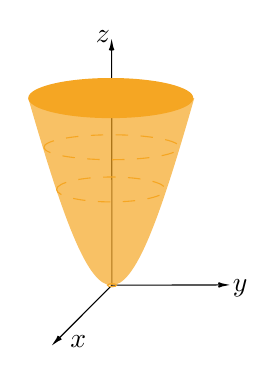
\begin{tikzpicture}[x=0.5pt,y=0.5pt,yscale=-1,xscale=1]
                        %Straight Lines [id:da9108779740102381] 
                        \draw    (130.5,219.74) -- (130.27,47.62) ;
                        \draw [shift={(130.26,45.62)}, rotate = 89.92] [color={rgb, 255:red, 0; green, 0; blue, 0 }  ][line width=0.75]    (4.37,-1.32) .. controls (2.78,-0.56) and (1.32,-0.12) .. (0,0) .. controls (1.32,0.12) and (2.78,0.56) .. (4.37,1.32)   ;
                        %Straight Lines [id:da1533658609071583] 
                        \draw    (130.5,219.74) -- (209.8,219.55) ;
                        \draw [shift={(211.8,219.55)}, rotate = 179.87] [color={rgb, 255:red, 0; green, 0; blue, 0 }  ][line width=0.75]    (4.37,-1.32) .. controls (2.78,-0.56) and (1.32,-0.12) .. (0,0) .. controls (1.32,0.12) and (2.78,0.56) .. (4.37,1.32)   ;
                        %Straight Lines [id:da4747079547908387] 
                        \draw    (130.5,219.74) -- (91.21,259.13) ;
                        \draw [shift={(89.8,260.55)}, rotate = 314.92] [color={rgb, 255:red, 0; green, 0; blue, 0 }  ][line width=0.75]    (4.37,-1.32) .. controls (2.78,-0.56) and (1.32,-0.12) .. (0,0) .. controls (1.32,0.12) and (2.78,0.56) .. (4.37,1.32)   ;
                        %Curve Lines [id:da8700830614722878] 
                        \draw [draw opacity=0][fill={rgb, 255:red, 245; green, 166; blue, 35 }  ,fill opacity=0.7 ]   (70,84.5) .. controls (121.8,264.45) and (138.5,265.5) .. (190,84.5) ;
                        %Flowchart: Connector [id:dp9931822219792372] 
                        \draw  [draw opacity=0][fill={rgb, 255:red, 245; green, 166; blue, 35 }  ,fill opacity=1 ] (70,84.5) .. controls (70,76.49) and (96.71,70) .. (129.65,70) .. controls (162.59,70) and (189.3,76.49) .. (189.3,84.5) .. controls (189.3,92.51) and (162.59,99) .. (129.65,99) .. controls (96.71,99) and (70,92.51) .. (70,84.5) -- cycle ;
                        %Flowchart: Connector [id:dp6783816821687585] 
                        \draw  [color={rgb, 255:red, 245; green, 166; blue, 35 }  ,draw opacity=1 ][dash pattern={on 4.5pt off 4.5pt}] (90.5,150.55) .. controls (90.5,145.58) and (108.14,141.55) .. (129.9,141.55) .. controls (151.66,141.55) and (169.3,145.58) .. (169.3,150.55) .. controls (169.3,155.52) and (151.66,159.55) .. (129.9,159.55) .. controls (108.14,159.55) and (90.5,155.52) .. (90.5,150.55) -- cycle ;
                        %Flowchart: Connector [id:dp5158806159989833] 
                        \draw  [color={rgb, 255:red, 245; green, 166; blue, 35 }  ,draw opacity=1 ][dash pattern={on 4.5pt off 4.5pt}] (81.3,120.05) .. controls (81.3,115.08) and (103.24,111.05) .. (130.3,111.05) .. controls (157.36,111.05) and (179.3,115.08) .. (179.3,120.05) .. controls (179.3,125.02) and (157.36,129.05) .. (130.3,129.05) .. controls (103.24,129.05) and (81.3,125.02) .. (81.3,120.05) -- cycle ;
                        %Flowchart: Connector [id:dp7285429676748697] 
                        \draw  [color={rgb, 255:red, 245; green, 166; blue, 35 }  ,draw opacity=1 ] (127.3,219.74) .. controls (127.3,219.12) and (128.76,218.61) .. (130.55,218.61) .. controls (132.34,218.61) and (133.8,219.12) .. (133.8,219.74) .. controls (133.8,220.36) and (132.34,220.86) .. (130.55,220.86) .. controls (128.76,220.86) and (127.3,220.36) .. (127.3,219.74) -- cycle ;

                        % Text Node
                        \draw (98.54,254.3) node [anchor=north west][inner sep=0.75pt]  [font=\normalsize]  {$x$};
                        % Text Node
                        \draw (215.96,214.03) node [anchor=north west][inner sep=0.75pt]  [font=\normalsize]  {$y$};
                        % Text Node
                        \draw (116.96,34.03) node [anchor=north west][inner sep=0.75pt]  [font=\normalsize]  {$z$};
                    \end{tikzpicture}
                \caption{\(f(x,y) = \frac{x^2 + 2x^2y^2 + y^2}{x^2 + y^2}\)}
                \label{fig:Limte0}
        \end{figure}
    geometricamente vemos que, quando \((x,y)\) se aproxima de \((0,0)\), \(f(x,y)\) se aproxima de zero.
\end{example}

Em geral, se uma função \(f\) está definida num conjunto aberto contendo um ponto \((x_0,y_0)\), exceto, possivelmente, em \((x_0,y_0)\) podemos perguntar:
    {\begin{center}
        ``O valor de \(f(x,y)\) pode ficar tão próximo de \(L\in\R\) quanto queiramos, escolhendo \((x,y)\) suficientemente próximo de \((x_0,y_0)\)?''
    \end{center}}
Ou ainda,
    {\begin{center}
        A medida que \((x,y)\) se aproxima de \((x_0,y_0)\) (mas \((x,y)\neq(x_0,y_0)\)), \(f(x,y)\) tende a \(L\in\R\)?
    \end{center}}
Quando a resposta é \textit{sim}, escrevemos \[\lim_{(x,y)\to(x_0,y_0)} f(x,y) = L\] e dizemos que o limite de \(f(x,y)\) quando \((x,y)\) tende a \((x_0,y_0)\) é \(L\).

Usando esta notação para o exemplo anterior, \[\lim_{(x,y)\to(0,0)} \frac{x^4 + 2x^2y^2 + y^2}{x^2 + y^2} = 0.\]

A seguir formalizamos a ideia de limite na seguinte definição:
\begin{definition}
    Sejam \(f:D_f\subset\R^2 \to \R\), \((x_0,y_0)\) um ponto de acumulação de \(D_f\) e \(L\in\R\). Definimos \[\lim_{(x,y)\to(x_0,y_0)} f(x,y) = L\] se, para todo \(\varepsilon>0\), existe \(\delta>0\) tal que, para todo \((x,y)\in D_f\), \[(x,y)\in D_f, \text{ e } 0 < \|(x,y)-(x_0,y_0)\| < \delta \Rightarrow |f(x,y) - L| < \delta.\]\index{Funções de duas variáveis a valores reais! Limite}
            \begin{figure}[htbp]
                \centering
                    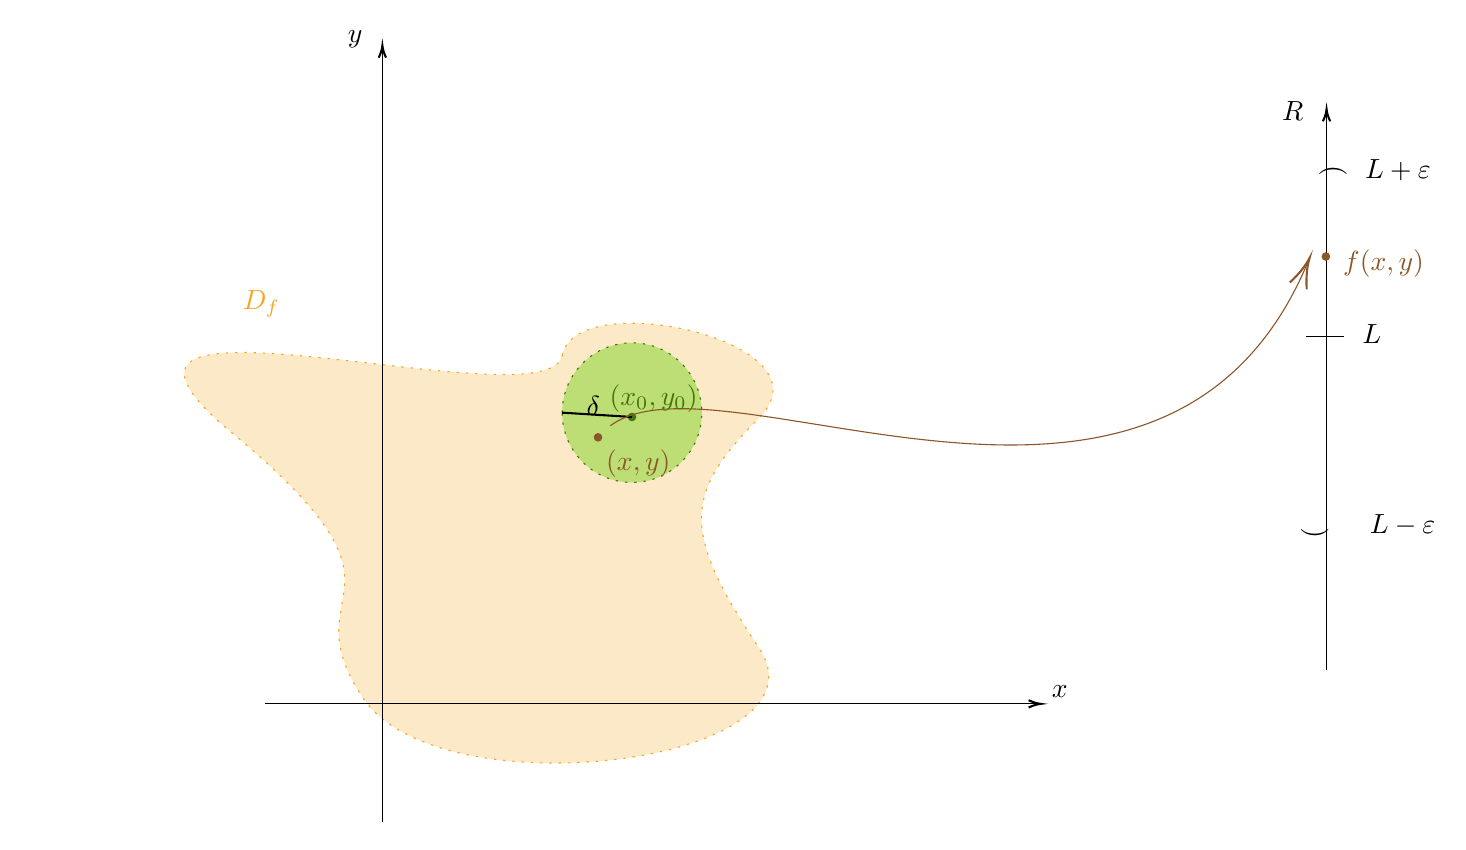
\begin{tikzpicture}[x=1pt,y=1pt,yscale=-1,xscale=1]
                        %Shape: Polygon Curved [id:ds9927915703986574] 
                        \draw  [color={rgb, 255:red, 245; green, 166; blue, 35 }  ,draw opacity=1 ][fill={rgb, 255:red, 245; green, 166; blue, 35 }  ,fill opacity=0.25 ][dash pattern={on 0.84pt off 2.51pt}] (144.59,126.75) .. controls (149.43,101.16) and (243.34,121.7) .. (215.68,149.36) .. controls (188.02,177.02) and (188.02,190.85) .. (215.68,232.35) .. controls (243.34,273.84) and (100.33,292.02) .. (72.67,250.53) .. controls (45.01,209.04) and (98.26,215.26) .. (24.96,154.41) .. controls (-48.35,93.55) and (139.75,152.33) .. (144.59,126.75) -- cycle ;
                        %Shape: Ellipse [id:dp13909363038935796] 
                        \draw  [color={rgb, 255:red, 65; green, 117; blue, 5 }  ,draw opacity=1 ][fill={rgb, 255:red, 126; green, 211; blue, 33 }  ,fill opacity=0.5 ][dash pattern={on 0.84pt off 2.51pt}] (144.6,147.39) .. controls (144.6,133.46) and (155.89,122.16) .. (169.82,122.16) .. controls (183.75,122.16) and (195.05,133.46) .. (195.05,147.39) .. controls (195.05,161.32) and (183.75,172.61) .. (169.82,172.61) .. controls (155.89,172.61) and (144.6,161.32) .. (144.6,147.39) -- cycle ;
                        %Shape: Ellipse [id:dp9318127719685116] 
                        \draw  [draw opacity=0][fill={rgb, 255:red, 65; green, 117; blue, 5 }  ,fill opacity=1 ] (168.26,148.95) .. controls (168.26,148.09) and (168.96,147.39) .. (169.82,147.39) .. controls (170.69,147.39) and (171.38,148.09) .. (171.38,148.95) .. controls (171.38,149.81) and (170.69,150.51) .. (169.82,150.51) .. controls (168.96,150.51) and (168.26,149.81) .. (168.26,148.95) -- cycle ;
                        %Shape: Ellipse [id:dp7313855451597336] 
                        \draw  [draw opacity=0][fill={rgb, 255:red, 139; green, 87; blue, 42 }  ,fill opacity=1 ] (155.99,156.31) .. controls (155.99,155.45) and (156.69,154.75) .. (157.55,154.75) .. controls (158.41,154.75) and (159.11,155.45) .. (159.11,156.31) .. controls (159.11,157.17) and (158.41,157.87) .. (157.55,157.87) .. controls (156.69,157.87) and (155.99,157.17) .. (155.99,156.31) -- cycle ;
                        %Straight Lines [id:da6073611479159446] 
                        \draw [line width=0.75]    (144.6,147.39) -- (169.82,148.95) ;
                        %Straight Lines [id:da21092003680750693] 
                        \draw    (79.63,295.22) -- (79.63,16.74) ;
                        \draw [shift={(79.63,14.74)}, rotate = 90] [color={rgb, 255:red, 0; green, 0; blue, 0 }  ][line width=0.75]    (4.37,-1.32) .. controls (2.78,-0.56) and (1.32,-0.12) .. (0,0) .. controls (1.32,0.12) and (2.78,0.56) .. (4.37,1.32)   ;
                        %Straight Lines [id:da007087146182350623] 
                        \draw    (37.04,252.62) -- (315.52,252.62) ;
                        \draw [shift={(317.52,252.62)}, rotate = 180] [color={rgb, 255:red, 0; green, 0; blue, 0 }  ][line width=0.75]    (4.37,-1.32) .. controls (2.78,-0.56) and (1.32,-0.12) .. (0,0) .. controls (1.32,0.12) and (2.78,0.56) .. (4.37,1.32)   ;
                        %Straight Lines [id:da2863727475115555] 
                        \draw    (420.8,240.52) -- (420.8,39.73) ;
                        \draw [shift={(420.8,37.73)}, rotate = 90] [color={rgb, 255:red, 0; green, 0; blue, 0 }  ][line width=0.75]    (4.37,-1.32) .. controls (2.78,-0.56) and (1.32,-0.12) .. (0,0) .. controls (1.32,0.12) and (2.78,0.56) .. (4.37,1.32)   ;
                        %Straight Lines [id:da6449937360990341] 
                        \draw    (413.2,119.9) -- (427.2,119.9) ;
                        %Shape: Ellipse [id:dp5714638045100543] 
                        \draw  [draw opacity=0][fill={rgb, 255:red, 139; green, 87; blue, 42 }  ,fill opacity=1 ] (418.99,90.98) .. controls (418.99,90.12) and (419.69,89.42) .. (420.55,89.42) .. controls (421.41,89.42) and (422.11,90.12) .. (422.11,90.98) .. controls (422.11,91.84) and (421.41,92.54) .. (420.55,92.54) .. controls (419.69,92.54) and (418.99,91.84) .. (418.99,90.98) -- cycle ;
                        %Curve Lines [id:da3820597792677821] 
                        \draw [color={rgb, 255:red, 139; green, 87; blue, 42 }  ,draw opacity=1 ]   (162,152.13) .. controls (202,122.13) and (363.33,218.13) .. (414.67,91.47) ;
                        \draw [shift={(414.67,91.47)}, rotate = 112.06] [color={rgb, 255:red, 139; green, 87; blue, 42 }  ,draw opacity=1 ][line width=0.75]    (10.93,-3.29) .. controls (6.95,-1.4) and (3.31,-0.3) .. (0,0) .. controls (3.31,0.3) and (6.95,1.4) .. (10.93,3.29)   ;

                        % Text Node
                        \draw (320.61,245.13) node [anchor=north west][inner sep=0.75pt]  [font=\normalsize]  {$x$};
                        % Text Node
                        \draw (66.17,8.48) node [anchor=north west][inner sep=0.75pt]  [font=\normalsize]  {$y$};
                        % Text Node
                        \draw (403.81,33.99) node [anchor=north west][inner sep=0.75pt]  [font=\normalsize]  {$\mathbb{R}$};
                        % Text Node
                        \draw (28.23,102.42) node [anchor=north west][inner sep=0.75pt]  [font=\normalsize]  {$\textcolor[rgb]{0.96,0.65,0.14}{D_{f}}$};
                        % Text Node
                        \draw (160.78,136.27) node [anchor=north west][inner sep=0.75pt]  [font=\normalsize,color={rgb, 255:red, 65; green, 117; blue, 5 }  ,opacity=1 ]  {$( x_{0} ,y_{0})$};
                        % Text Node
                        \draw (159.55,159.71) node [anchor=north west][inner sep=0.75pt]  [font=\normalsize,color={rgb, 255:red, 139; green, 87; blue, 42 }  ,opacity=1 ]  {$( x,y)$};
                        % Text Node
                        \draw (152.44,140.49) node [anchor=north west][inner sep=0.75pt]  [font=\normalsize]  {$\delta $};
                        % Text Node
                        \draw (432.8,114.47) node [anchor=north west][inner sep=0.75pt]  [font=\normalsize]  {$L$};
                        % Text Node
                        \draw (429.07,57.07) node [anchor=north west][inner sep=0.75pt]  [rotate=-90]  {$($};
                        % Text Node
                        \draw (410.53,193.73) node [anchor=north west][inner sep=0.75pt]  [rotate=-270]  {$($};
                        % Text Node
                        \draw (435.47,183.13) node [anchor=north west][inner sep=0.75pt]  [font=\normalsize]  {$L-\varepsilon $};
                        % Text Node
                        \draw (433.8,55.07) node [anchor=north west][inner sep=0.75pt]  [font=\normalsize]  {$L+\varepsilon $};
                        % Text Node
                        \draw (425.88,87.73) node [anchor=north west][inner sep=0.75pt]  [font=\normalsize,color={rgb, 255:red, 139; green, 87; blue, 42 }  ,opacity=1 ]  {$f( x,y)$};
                    \end{tikzpicture}
                \caption{Limte}
                \label{fig:Limte}
            \end{figure}
\end{definition}

Em outras palavras, \(f(x,y)\) permanece em \((L-\varepsilon,L+\varepsilon)\) quando \((x,y)\in D_f\) \(((x,y)\neq(x_0,y_0))\) varia na bola aberta de centro \((x_0,y_0)\) e raio \(\delta\).

A partir de agora, quando falarmos que \(f\) tem limite em \((x_0,y_0)\), fica subentendido que \((x_0,y_0)\) é um ponto de acumulação de \(D_f\).

Às vezes, podemos denotar o limite por \[\lim_{\substack{x\to x_0 \\ y\to y_0}} f(x,y) = l \text{ ou } f(x,y) \xrightarrow{(x,y) \to (x_0,y_0)} L.\]

\begin{example}
    Se \(f(x,y) = 4\), então, para todo \((x_0,y_0)\in\R^2\), \(\displaystyle\lim_{\substack{x\to x_0 \\ y\to y_0}} f(x,y) = 4\).

    De fato, dado \(\varepsilon>0\), temos que encontrar \(\delta>0\) tal que, se \(0\leq \|(x,y)-(x_0,y_0)\| < \delta\), então \(|f(x,y) - 4| < \varepsilon\). Agora, note que \[|f(x,y) - 4| = |4 - 4| = 0 < \varepsilon.\] Portanto podemos tomar qualquer \(\delta>0\) para que \[0<\|(x,y) - (x_0,y_0)\|<\delta \Rightarrow |f(x,y) - 4| < \varepsilon.\]
\end{example}

\begin{exercise}
    Seja \(f(x,y) = k\in\R\). Mostre que \(\displaystyle\lim_{\substack{x\to x_0 \\ y\to y_0}} f(x,y) = k\).
\end{exercise}

\begin{example}
    Seja \(f(x,y) = x\). Então, para todo \((x_0,y_0)\in\R^2\), \(\displaystyle\lim_{\substack{x\to x_0 \\ y\to y_0}} f(x,y) = x_0\). De fato, dato \(\varepsilon>0\), queremos encontrar \(\delta>0\) tal que \[0<\|(x,y) - (x_0,y_0)\| < \delta \Rightarrow |f(x,y) - x_0| < \varepsilon.\] Para isso note que \[|f(x,y) - x_0| = |x - x_0| = \sqrt{(x-x_0)^2} \leq \sqrt{(x-x_0)^2 + (y-y_0)^2},\] portanto, tomando \(\delta = \varepsilon\) (ou \(\delta\leq \varepsilon\)), temos que \[0 < \|(x,y) - (x_0,y_0)\| < \delta = \varepsilon \Rightarrow |f(x,y) - x_0| < \varepsilon.\]
\end{example}

\begin{exercise}
    Seja \(f(x,y) = y\in\R\). Mostre que \(\displaystyle\lim_{\substack{x\to x_0 \\ y\to y_0}} f(x,y) = y_0\).
\end{exercise}

\begin{example}
    Considere \(f(x,y) = 3x + 7y\). Mostre que \(\displaystyle\lim_{\substack{x\to 2 \\ y\to 1}} f(x,y) = 13.\)

    Note primeiro que
        \begin{align*}
            |f(x,y) - 13|
                & = |(3x+7y) - 13| \\
                & = |(3x - 6) - (7y - 7)| \\
                & = |3(x-2) + 7(y-1)| \\
                & \leq 3|x-2| + 7|y-1| \\
                & \leq 3\sqrt{(x-2)^2} + 7\sqrt{(y-1)^2} \\
                & \leq 3\sqrt{(x-2)^2 + (y-1)^2} + 7\sqrt{(x-2)^2 + (y-1)^2} \\
                & = 10\sqrt{(x-2)^2 + (y-1)^2} = 10 \|(x,y) - (x_0,y_0)\| < 10 \delta.
        \end{align*}
    Assim, tomando \(\delta = \frac{\varepsilon}{10}\) (ou \(\delta\leq\frac{\varepsilon}{10}\)), temos \[0 < \|(x,y) - (x_0,y_0)\| < \frac{\varepsilon}{10} \Rightarrow |f(x,y) - 13| < 10\cdot\frac{\varepsilon}{10} = \varepsilon.\]
\end{example}

\begin{exercise}
    Mostre que \(\displaystyle\lim_{\substack{x\to x_0 \\ y\to y_0}} 3x + 2y = 7\).
\end{exercise}

\begin{example}
    Mostre que \(\displaystyle\lim_{\substack{x\to 0 \\ y\to 0}} \frac{2xy}{\sqrt{x^2 + y^2}} = 0\).

    Dado \(\varepsilon>0\), queremos encontrar \(\delta>0\) tal que \[0 < \|(x,y) - (0,0)\| = \sqrt{x^2 + y^2} < \delta \Rightarrow \left|\frac{2xy}{\sqrt{x^2 + y^2}} - 0\right| < \varepsilon.\] Mas
        \begin{align*}
            \left|\frac{2xy}{\sqrt{x^2 + y^2}}\right|
                & = \frac{2|x||y|}{\sqrt{x^2 + y^2}} \\
                & = \frac{2\sqrt{x^2}\sqrt{y^2}}{\sqrt{x^2+y^2}} \\
                & \leq \frac{2\sqrt{x^2 + y^2}\sqrt{x^2 + y^2}}{\sqrt{x^2+y^2}} \\
                & = 2\sqrt{x^2+y^2} = 2\|(x,y)\| < 2\delta,
        \end{align*}
    portanto, tomando \(\delta = \frac{\varepsilon}{2}\), temos \[\|(x,y)\| < \frac{\varepsilon}{2} \Rightarrow \left|\frac{2xy}{\sqrt{x^2 + y ^2}}\right| < \varepsilon\]
\end{example}

Para uma função de uma única variável real, existem apenas duas formas de aproximação do ponto \(x = x_0\): ou pela direita, ou pela esquerda. Mais ainda, sabemos que \[\lim_{x\to x_0} f(x) = L \Leftrightarrow \lim_{x\to x_0^+} f(x) = L = \lim_{x\to x_0^-} f(x).\]

Agora, para funções de duas (ou mais) variáveis, temos infinitas formas de aproximar do ponto \((x_0,y_0)\).
    \begin{figure}[htbp]
        \centering
            \begin{tikzpicture}[x=0.5pt,y=0.5pt,yscale=-1,xscale=1]
                %Shape: Ellipse [id:dp6735342190837837] 
                \draw  [draw opacity=0][fill={rgb, 255:red, 245; green, 166; blue, 35 }  ,fill opacity=1 ] (342.2,139.82) .. controls (342.2,135.48) and (345.72,131.97) .. (350.06,131.97) .. controls (354.4,131.97) and (357.91,135.48) .. (357.91,139.82) .. controls (357.91,144.16) and (354.4,147.68) .. (350.06,147.68) .. controls (345.72,147.68) and (342.2,144.16) .. (342.2,139.82) -- cycle ;
                %Curve Lines [id:da9110962211084549] 
                \draw    (114.34,116.72) .. controls (247.46,45.52) and (289.1,88.67) .. (317.35,114.01) ;
                \draw [shift={(318.63,115.15)}, rotate = 221.63] [color={rgb, 255:red, 0; green, 0; blue, 0 }  ][line width=0.75]    (4.37,-1.32) .. controls (2.78,-0.56) and (1.32,-0.12) .. (0,0) .. controls (1.32,0.12) and (2.78,0.56) .. (4.37,1.32)   ;
                %Curve Lines [id:da2448080649001152] 
                \draw    (214.91,119.39) .. controls (273.43,168.67) and (289.7,156.08) .. (311.03,140.76) ;
                \draw [shift={(312.34,139.82)}, rotate = 144.46] [color={rgb, 255:red, 0; green, 0; blue, 0 }  ][line width=0.75]    (4.37,-1.32) .. controls (2.78,-0.56) and (1.32,-0.12) .. (0,0) .. controls (1.32,0.12) and (2.78,0.56) .. (4.37,1.32)   ;
                %Curve Lines [id:da21428385042645148] 
                \draw    (216.48,223.58) .. controls (233.6,184.69) and (318.48,218.18) .. (327.8,174.64) ;
                \draw [shift={(328.06,173.29)}, rotate = 99.78] [color={rgb, 255:red, 0; green, 0; blue, 0 }  ][line width=0.75]    (4.37,-1.32) .. controls (2.78,-0.56) and (1.32,-0.12) .. (0,0) .. controls (1.32,0.12) and (2.78,0.56) .. (4.37,1.32)   ;
                %Curve Lines [id:da634869694261807] 
                \draw    (384.63,262.39) .. controls (307.23,223.7) and (376.21,212.44) .. (351.26,179.08) ;
                \draw [shift={(350.06,177.54)}, rotate = 50.71] [color={rgb, 255:red, 0; green, 0; blue, 0 }  ][line width=0.75]    (4.37,-1.32) .. controls (2.78,-0.56) and (1.32,-0.12) .. (0,0) .. controls (1.32,0.12) and (2.78,0.56) .. (4.37,1.32)   ;
                %Curve Lines [id:da33781733929475943] 
                \draw    (460.06,231.44) .. controls (431.77,143.44) and (416.06,317.87) .. (379.91,168.58) ;
                \draw [shift={(379.91,168.58)}, rotate = 76.39] [color={rgb, 255:red, 0; green, 0; blue, 0 }  ][line width=0.75]    (4.37,-1.32) .. controls (2.78,-0.56) and (1.32,-0.12) .. (0,0) .. controls (1.32,0.12) and (2.78,0.56) .. (4.37,1.32)   ;
                %Curve Lines [id:da8212319444209916] 
                \draw    (444.34,77.44) .. controls (334.44,32.55) and (322.12,75.63) .. (348.81,100.96) ;
                \draw [shift={(350.06,102.11)}, rotate = 221.63] [color={rgb, 255:red, 0; green, 0; blue, 0 }  ][line width=0.75]    (4.37,-1.32) .. controls (2.78,-0.56) and (1.32,-0.12) .. (0,0) .. controls (1.32,0.12) and (2.78,0.56) .. (4.37,1.32)   ;
                %Curve Lines [id:da7560469339428443] 
                \draw    (546.49,119.87) .. controls (441.73,127.68) and (420.98,48.38) .. (371.24,107.96) ;
                \draw [shift={(370.49,108.87)}, rotate = 309.37] [color={rgb, 255:red, 0; green, 0; blue, 0 }  ][line width=0.75]    (4.37,-1.32) .. controls (2.78,-0.56) and (1.32,-0.12) .. (0,0) .. controls (1.32,0.12) and (2.78,0.56) .. (4.37,1.32)   ;
                %Curve Lines [id:da4238194982639595] 
                \draw    (573.2,160.72) .. controls (468.97,168.5) and (430.96,113.13) .. (389.04,139.01) ;
                \draw [shift={(387.77,139.82)}, rotate = 326.75] [color={rgb, 255:red, 0; green, 0; blue, 0 }  ][line width=0.75]    (4.37,-1.32) .. controls (2.78,-0.56) and (1.32,-0.12) .. (0,0) .. controls (1.32,0.12) and (2.78,0.56) .. (4.37,1.32)   ;
                %Curve Lines [id:da11426524524740811] 
                \draw    (518.2,187.44) .. controls (414.49,195.18) and (426.66,158.7) .. (388,157.15) ;
                \draw [shift={(386.2,157.11)}, rotate = 0.66] [color={rgb, 255:red, 0; green, 0; blue, 0 }  ][line width=0.75]    (4.37,-1.32) .. controls (2.78,-0.56) and (1.32,-0.12) .. (0,0) .. controls (1.32,0.12) and (2.78,0.56) .. (4.37,1.32)   ;
            \end{tikzpicture}
        \caption{Caminhos}
        \label{fig:caminhos}
    \end{figure}
Mas a definiçao de limite se refere somente à distância entre \((x,y)\) e \((x_0,y_0)\), não se refere à direção de aproximação. Logo, se o limite existe, então \(f(x,y)\) deve se aproximar do mesmo valor limite ``independente'' do modo como \((x,y)\to(x_0,y_0)\). Assim, se \(f(x,y) \to L_1\) quando \((x,y) \to (x_0,y_0)\) através do caminho \(C_1\) e \(f(x,y) \to L_2\) quando \((x,y)\to(x_0,y_0)\) pelo caminho \(C_2\) e \(L_1 \neq L_2\), então \(\displaystyle\lim_{\substack{x\to 0 \\ y\to 0}} f(x,y)\) não existe.

\begin{example}
    Mostre que \(\displaystyle\lim_{\substack{x\to 0 \\ y\to 0}} \frac{x^2 - y^2}{x^2+y^2}\) não existe.

    Note que se \((x,y) \to (0,0)\) ao longo do eixo \(x\) (isto é, \(y=0\)), então \[\displaystyle\lim_{\substack{x\to 0 \\ y\to 0}} f(x,y) = \displaystyle\lim_{\substack{x\to 0}} f(x,0) = \frac{x^2}{x^2} = 1.\] Por outro lado, se \((x,y) \to (0,0)\) ao longo do eixo \(y\) (\(x=0\)), então \[\displaystyle\lim_{\substack{x\to 0 \\ y\to 0}} f(x,y) = \displaystyle\lim_{\substack{y\to 0}} f(0,y) = \frac{-y^2}{y^2} = -1.\] Ou seja, \(\lim_{(x,y)\to(0,0)} f(x,y) = 1\) quando \((x,y) to (0,0)\) pelo caminho \(y=0\), e \(\lim_{(x,y)\to(0,0)} f(x,y) = -1\) quando \((x,y) to (0,0)\) pelo caminho \(x=0\). Portanto o limite não existe.
\end{example}

\begin{example}
    Calcule, se existir, \(\displaystyle\lim_{\substack{x\to 0 \\ y\to 0}} \frac{xy}{x^2+y^2}\).

    Note que, se \(y = 0\), então \[\displaystyle\lim_{\substack{x\to 0 \\ y\to 0}} f(x,y) = \displaystyle\lim_{\substack{x\to 0}} f(x,0) = \frac{0}{x^2} = 0.\] Também, se \(x = 0\), \[\displaystyle\lim_{\substack{x\to 0 \\ y\to 0}} f(x,y) = \displaystyle\lim_{\substack{y\to 0}} f(0,y) = \frac{0}{y^2} = 0.\] Para estes dois caminhos, então, temos que \(\lim_{(x,y) \to (0,0)} f(x,y) = 0\). Podemos concluir que \(\displaystyle\lim_{\substack{x\to 0 \\ y\to 0}} \frac{xy}{x^2+y^2} = 0\)?
        \begin{figure}[htbp]
            \centering
                \begin{tikzpicture}[x=0.5pt,y=0.5pt,yscale=-1,xscale=1]
                    %Straight Lines [id:da7751809194408749] 
                    \draw    (337.78,272.49) -- (337.78,18.76) ;
                    \draw [shift={(337.78,16.76)}, rotate = 90] [color={rgb, 255:red, 0; green, 0; blue, 0 }  ][line width=0.75]    (4.37,-1.32) .. controls (2.78,-0.56) and (1.32,-0.12) .. (0,0) .. controls (1.32,0.12) and (2.78,0.56) .. (4.37,1.32)   ;
                    %Straight Lines [id:da4225866159104621] 
                    \draw    (203.2,140.36) -- (456.93,140.36) ;
                    \draw [shift={(458.93,140.36)}, rotate = 180] [color={rgb, 255:red, 0; green, 0; blue, 0 }  ][line width=0.75]    (4.37,-1.32) .. controls (2.78,-0.56) and (1.32,-0.12) .. (0,0) .. controls (1.32,0.12) and (2.78,0.56) .. (4.37,1.32)   ;
                    %Straight Lines [id:da5556238563442709] 
                    \draw [color={rgb, 255:red, 208; green, 2; blue, 27 }  ,draw opacity=1 ]   (203.2,140.36) -- (329.07,140.36) ;
                    \draw [shift={(331.07,140.36)}, rotate = 180] [color={rgb, 255:red, 208; green, 2; blue, 27 }  ,draw opacity=1 ][line width=0.75]    (10.93,-3.29) .. controls (6.95,-1.4) and (3.31,-0.3) .. (0,0) .. controls (3.31,0.3) and (6.95,1.4) .. (10.93,3.29)   ;
                    %Straight Lines [id:da050913708442122174] 
                    \draw [color={rgb, 255:red, 208; green, 2; blue, 27 }  ,draw opacity=1 ]   (458.93,140.36) -- (346.67,140.27) ;
                    \draw [shift={(344.67,140.27)}, rotate = 0.05] [color={rgb, 255:red, 208; green, 2; blue, 27 }  ,draw opacity=1 ][line width=0.75]    (10.93,-3.29) .. controls (6.95,-1.4) and (3.31,-0.3) .. (0,0) .. controls (3.31,0.3) and (6.95,1.4) .. (10.93,3.29)   ;
                    %Straight Lines [id:da5197441959309841] 
                    \draw [color={rgb, 255:red, 65; green, 117; blue, 5 }  ,draw opacity=1 ]   (337.78,272.49) -- (337.78,146.62) ;
                    \draw [shift={(337.78,144.62)}, rotate = 90] [color={rgb, 255:red, 65; green, 117; blue, 5 }  ,draw opacity=1 ][line width=0.75]    (10.93,-3.29) .. controls (6.95,-1.4) and (3.31,-0.3) .. (0,0) .. controls (3.31,0.3) and (6.95,1.4) .. (10.93,3.29)   ;
                    %Straight Lines [id:da5710399662533471] 
                    \draw [color={rgb, 255:red, 65; green, 117; blue, 5 }  ,draw opacity=1 ]   (338,21.6) -- (338,134.27) ;
                    \draw [shift={(338,136.27)}, rotate = 270] [color={rgb, 255:red, 65; green, 117; blue, 5 }  ,draw opacity=1 ][line width=0.75]    (10.93,-3.29) .. controls (6.95,-1.4) and (3.31,-0.3) .. (0,0) .. controls (3.31,0.3) and (6.95,1.4) .. (10.93,3.29)   ;
                    %Straight Lines [id:da008109240882351876] 
                    \draw [color={rgb, 255:red, 74; green, 144; blue, 226 }  ,draw opacity=1 ]   (220.1,260.28) -- (328.44,151.69) ;
                    \draw [shift={(329.85,150.27)}, rotate = 134.93] [color={rgb, 255:red, 74; green, 144; blue, 226 }  ,draw opacity=1 ][line width=0.75]    (10.93,-3.29) .. controls (6.95,-1.4) and (3.31,-0.3) .. (0,0) .. controls (3.31,0.3) and (6.95,1.4) .. (10.93,3.29)   ;
                    %Straight Lines [id:da49600441836662035] 
                    \draw [color={rgb, 255:red, 74; green, 144; blue, 226 }  ,draw opacity=1 ]   (440.1,40.65) -- (351.77,128.86) ;
                    \draw [shift={(350.35,130.27)}, rotate = 315.04] [color={rgb, 255:red, 74; green, 144; blue, 226 }  ,draw opacity=1 ][line width=0.75]    (10.93,-3.29) .. controls (6.95,-1.4) and (3.31,-0.3) .. (0,0) .. controls (3.31,0.3) and (6.95,1.4) .. (10.93,3.29)   ;

                    % Text Node
                    \draw (461.23,133.03) node [anchor=north west][inner sep=0.75pt]  [font=\footnotesize]  {$x$};
                    % Text Node
                    \draw (324.97,10.56) node [anchor=north west][inner sep=0.75pt]  [font=\footnotesize]  {$y$};
                    % Text Node
                    \draw (415.73,144.07) node [anchor=north west][inner sep=0.75pt]    {$\textcolor[rgb]{0.82,0.01,0.11}{x=0}$};
                    % Text Node
                    \draw (345.07,25.4) node [anchor=north west][inner sep=0.75pt]    {$\textcolor[rgb]{0.25,0.46,0.02}{y=0}$};
                    % Text Node
                    \draw (420.1,59.9) node [anchor=north west][inner sep=0.75pt]    {$\textcolor[rgb]{0.29,0.56,0.89}{y=x}$};
                \end{tikzpicture}
            \caption{\(\lim_{\substack{x\to 0 \\ y\to 0}} \frac{xy}{x^2+y^2}\)}
            \label{fig:limite1}
        \end{figure}
    Não! Note que, para o caminho \(x=y\), \(\displaystyle\lim_{\substack{x\to 0 \\ y\to 0}} \frac{xy}{x^2+y^2} = \lim_{x\to 0} \frac{x^2}{2x^2} = \frac{1}{2} \neq 0.\)
\end{example}

\begin{example}
    Calcule, se existir, \(\displaystyle\lim_{\substack{x\to 0 \\ y\to 0}} \frac{xy^2}{x^2+y^4}\).

    Observe que
        \begin{itemize}
            \item Se \(x=0\), então \[\lim_{\substack{x\to 0 \\ y\to 0}} \frac{xy^2}{x^2+y^4} = \lim_{\substack{y\to 0}} \frac{0}{y^4} = 0.\]
            \item Se \(y=0\), então \[\lim_{\substack{x\to 0 \\ y\to 0}} \frac{xy^2}{x^2+y^4} = \lim_{\substack{x\to 0}} \frac{0}{x^2} = 0.\]
            \item Se \(x=y\), então \[\lim_{\substack{x\to 0 \\ y\to 0}} \frac{xy^2}{x^2+y^4} = \lim_{\substack{x\to 0}} \frac{x^3}{x^2+x^4} = \lim_{x\to 0} \frac{x^3}{x^2(1+x^2)} = 0.\]
            \item Em geral, Se \(y = ax\), para algum \(a\in\R\), então \[\lim_{\substack{x\to 0 \\ y\to 0}} \frac{xy^2}{x^2+y^4} = \lim_{\substack{x\to 0}} \frac{x(ax)^2}{x^2 + (ax^4)} = \lim_{x\to 0} \frac{a^2 x^3}{x^2(1+a^4x^2)} = \lim_{x\to 0} \frac{a^2x}{1+a^4x^2} = 0.\]
            \item Porém, se \(x=y^2\) temos \[\lim_{\substack{x\to 0 \\ y\to 0}} \frac{xy^2}{x^2+y^4} = \lim_{y\to 0} \frac{y^2y^2}{y^2+y^4} = \lim_{y\to 0} \frac{y^4}{2y^4} = \frac{1}{2}. \] Portanto o limite não existe.
        \end{itemize}
        \begin{figure}[htbp]
            \centering
                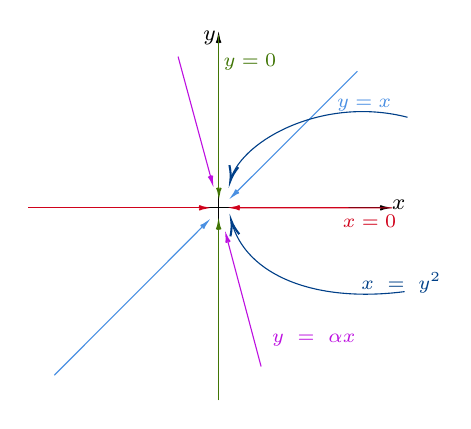
\begin{tikzpicture}[x=0.5pt,y=0.5pt,yscale=-1,xscale=1]
                    %Straight Lines [id:da6315767173422226] 
                    \draw    (169.78,292) -- (169.78,38.27) ;
                    \draw [shift={(169.78,36.27)}, rotate = 90] [color={rgb, 255:red, 0; green, 0; blue, 0 }  ][line width=0.75]    (4.37,-1.32) .. controls (2.78,-0.56) and (1.32,-0.12) .. (0,0) .. controls (1.32,0.12) and (2.78,0.56) .. (4.37,1.32)   ;
                    %Straight Lines [id:da18300736492834668] 
                    \draw    (35.2,159.86) -- (288.93,159.86) ;
                    \draw [shift={(290.93,159.86)}, rotate = 180] [color={rgb, 255:red, 0; green, 0; blue, 0 }  ][line width=0.75]    (4.37,-1.32) .. controls (2.78,-0.56) and (1.32,-0.12) .. (0,0) .. controls (1.32,0.12) and (2.78,0.56) .. (4.37,1.32)   ;
                    %Straight Lines [id:da05657850493305738] 
                    \draw [color={rgb, 255:red, 208; green, 2; blue, 27 }  ,draw opacity=1 ]   (32.2,159.86) -- (158.07,159.86) ;
                    \draw [shift={(160.07,159.86)}, rotate = 180] [color={rgb, 255:red, 208; green, 2; blue, 27 }  ,draw opacity=1 ][line width=0.75]    (4.37,-1.32) .. controls (2.78,-0.56) and (1.32,-0.12) .. (0,0) .. controls (1.32,0.12) and (2.78,0.56) .. (4.37,1.32)   ;
                    %Straight Lines [id:da8552927473524634] 
                    \draw [color={rgb, 255:red, 208; green, 2; blue, 27 }  ,draw opacity=1 ]   (294.93,159.86) -- (182.67,159.78) ;
                    \draw [shift={(180.67,159.77)}, rotate = 0.05] [color={rgb, 255:red, 208; green, 2; blue, 27 }  ,draw opacity=1 ][line width=0.75]    (4.37,-1.32) .. controls (2.78,-0.56) and (1.32,-0.12) .. (0,0) .. controls (1.32,0.12) and (2.78,0.56) .. (4.37,1.32)   ;
                    %Straight Lines [id:da6655716295466797] 
                    \draw [color={rgb, 255:red, 65; green, 117; blue, 5 }  ,draw opacity=1 ]   (169.78,299) -- (169.78,173.13) ;
                    \draw [shift={(169.78,171.13)}, rotate = 90] [color={rgb, 255:red, 65; green, 117; blue, 5 }  ,draw opacity=1 ][line width=0.75]    (4.37,-1.32) .. controls (2.78,-0.56) and (1.32,-0.12) .. (0,0) .. controls (1.32,0.12) and (2.78,0.56) .. (4.37,1.32)   ;
                    %Straight Lines [id:da3613444125360147] 
                    \draw [color={rgb, 255:red, 65; green, 117; blue, 5 }  ,draw opacity=1 ]   (170,35.11) -- (170,147.77) ;
                    \draw [shift={(170,149.77)}, rotate = 270] [color={rgb, 255:red, 65; green, 117; blue, 5 }  ,draw opacity=1 ][line width=0.75]    (4.37,-1.32) .. controls (2.78,-0.56) and (1.32,-0.12) .. (0,0) .. controls (1.32,0.12) and (2.78,0.56) .. (4.37,1.32)   ;
                    %Straight Lines [id:da20740276792348855] 
                    \draw [color={rgb, 255:red, 74; green, 144; blue, 226 }  ,draw opacity=1 ]   (51.1,280.78) -- (159.44,172.2) ;
                    \draw [shift={(160.85,170.78)}, rotate = 134.93] [color={rgb, 255:red, 74; green, 144; blue, 226 }  ,draw opacity=1 ][line width=0.75]    (4.37,-1.32) .. controls (2.78,-0.56) and (1.32,-0.12) .. (0,0) .. controls (1.32,0.12) and (2.78,0.56) .. (4.37,1.32)   ;
                    %Straight Lines [id:da4743580207569783] 
                    \draw [color={rgb, 255:red, 74; green, 144; blue, 226 }  ,draw opacity=1 ]   (270.1,61.16) -- (181.77,149.37) ;
                    \draw [shift={(180.35,150.78)}, rotate = 315.04] [color={rgb, 255:red, 74; green, 144; blue, 226 }  ,draw opacity=1 ][line width=0.75]    (4.37,-1.32) .. controls (2.78,-0.56) and (1.32,-0.12) .. (0,0) .. controls (1.32,0.12) and (2.78,0.56) .. (4.37,1.32)   ;
                    %Straight Lines [id:da33441609244936643] 
                    \draw [color={rgb, 255:red, 189; green, 16; blue, 224 }  ,draw opacity=1 ]   (140.5,50.55) -- (164.48,139.12) ;
                    \draw [shift={(165,141.05)}, rotate = 254.85] [color={rgb, 255:red, 189; green, 16; blue, 224 }  ,draw opacity=1 ][line width=0.75]    (4.37,-1.32) .. controls (2.78,-0.56) and (1.32,-0.12) .. (0,0) .. controls (1.32,0.12) and (2.78,0.56) .. (4.37,1.32)   ;
                    %Straight Lines [id:da6915781797168352] 
                    \draw [color={rgb, 255:red, 189; green, 16; blue, 224 }  ,draw opacity=1 ]   (200.5,274.55) -- (176.01,182.48) ;
                    \draw [shift={(175.5,180.55)}, rotate = 75.11] [color={rgb, 255:red, 189; green, 16; blue, 224 }  ,draw opacity=1 ][line width=0.75]    (4.37,-1.32) .. controls (2.78,-0.56) and (1.32,-0.12) .. (0,0) .. controls (1.32,0.12) and (2.78,0.56) .. (4.37,1.32)   ;
                    %Curve Lines [id:da7177904687879447] 
                    \draw [color={rgb, 255:red, 0; green, 63; blue, 136 }  ,draw opacity=1 ]   (306.27,94.4) .. controls (245.51,78.72) and (187.31,111.06) .. (178.73,138.71) ;
                    \draw [shift={(178.27,140.4)}, rotate = 283.39] [color={rgb, 255:red, 0; green, 63; blue, 136 }  ,draw opacity=1 ][line width=0.75]    (10.93,-3.29) .. controls (6.95,-1.4) and (3.31,-0.3) .. (0,0) .. controls (3.31,0.3) and (6.95,1.4) .. (10.93,3.29)   ;
                    %Curve Lines [id:da6905840055818371] 
                    \draw [color={rgb, 255:red, 0; green, 63; blue, 136 }  ,draw opacity=1 ]   (304.27,220.4) .. controls (237.94,228.94) and (189.73,207.72) .. (179.38,170.77) ;
                    \draw [shift={(178.93,169.07)}, rotate = 76.2] [color={rgb, 255:red, 0; green, 63; blue, 136 }  ,draw opacity=1 ][line width=0.75]    (10.93,-3.29) .. controls (6.95,-1.4) and (3.31,-0.3) .. (0,0) .. controls (3.31,0.3) and (6.95,1.4) .. (10.93,3.29)   ;

                    % Text Node
                    \draw (293.23,152.54) node [anchor=north west][inner sep=0.75pt]  [font=\footnotesize]  {$x$};
                    % Text Node
                    \draw (156.97,30.06) node [anchor=north west][inner sep=0.75pt]  [font=\footnotesize]  {$y$};
                    % Text Node
                    \draw (257.73,163.07) node [anchor=north west][inner sep=0.75pt]  [font=\scriptsize]  {$\textcolor[rgb]{0.82,0.01,0.11}{x=0}$};
                    % Text Node
                    \draw (171.57,46.91) node [anchor=north west][inner sep=0.75pt]  [font=\scriptsize]  {$\textcolor[rgb]{0.25,0.46,0.02}{y=0}$};
                    % Text Node
                    \draw (253.6,79.41) node [anchor=north west][inner sep=0.75pt]  [font=\scriptsize]  {$\textcolor[rgb]{0.29,0.56,0.89}{y=x}$};
                    % Text Node
                    \draw (206.5,249.3) node [anchor=north west][inner sep=0.75pt]  [font=\scriptsize,color={rgb, 255:red, 189; green, 16; blue, 224 }  ,opacity=1 ]  {$y\ =\ \alpha x$};
                    % Text Node
                    \draw (271.07,204.41) node [anchor=north west][inner sep=0.75pt]  [font=\scriptsize]  {$\textcolor[rgb]{0,0.25,0.53}{x\ =\ y^{2}}$};
                \end{tikzpicture}
            \caption{\(\lim_{\substack{x\to 0 \\ y\to 0}} \frac{xy^2 }{x^2+y^2}\)}
            \label{fig:limite2}
        \end{figure}
\end{example}

\begin{exercise}
    Calcule, se existir, \(\lim_{(x,y)\to(0,0)} \frac{x-y}{2x+y}\).
\end{exercise}


\subsection{Propriedades básicas do limite}

As propriedades a seguir podem simplificar o cálculo do limite e suas demonstrações são análogas às demonstrações para funções de uma variável.
\begin{enumerate}
    \item (Teorema do sanduíche)\index{Teorema! do Sanduíche (Confronto)}: Se \(f(x,y) \leq g(x,y) \leq h(x,y)\) para \(0 < \|(x,y) - (x_0,y_0)\| < r\) e \[\lim_{(x,y)\to(x_0,y_0)} f(x,y) = L = \lim_{(x,y)\to (x_0,y_0)} h(x,y),\] então \(\lim_{(x,y)\to(x_0,y_0)} g(x,y) = L\).
    \item Se \(\lim_{(x,y)\to(x_0,y_0)} f(x,y) = 0\) e \(|g(x,y)| \leq M\) para \(0 < \|(x,y) - (x_0,y_0)\| < r\), então \[\lim_{(x,y)\to(x_0,y_0)} f(x)\cdot g(x) = 0.\]
    \item \(\lim_{(x,y)\to(x_0,y_0)} f(x,y) = 0 \Leftrightarrow \lim_{(x,y)\to(x_0,y_0)} |f(x,y)| = 0\).
    \item \(\lim_{(x,y)\to(x_0,y_0)} f(x,y) = L \Leftrightarrow \lim_{(x,y)\to(x_0,y_0)} (f(x,y) - L) = 0 \).
    \item \(\lim_{(x,y)\to(x_0,y_0)} f(x,y) = L \Leftrightarrow \lim_{(h,k)\to(0,0)} f(x_0 +h,y_0+k)\).
    \item Se \(\lim_{(x,y)\to(x_0,y_0)} f(x,y) = L\) e \(\lim_{(x,y)\to(x_0,y_0)} g(x,y)\), então
        \begin{enumerate}
            \item \(\lim_{(x,y)\to(x_0,y_0)} (f(x,y) + g(x,y)) = L + M\).
            \item \(\lim_{(x,y)\to(x_0,y_0)} K f(x,y) = KL\).
            \item \(\lim_{(x,y)\to(x_0,y_0)} f(x,y)\cdot g(x,y) = L\cdot M\).
            \item \(\lim_{(x,y)\to(x_0,y_0)} \frac{f(x,y)}{g(x,y)} = \frac{L}{M}\).
        \end{enumerate}
    \item (Conservação do sinal)\index{Teorema! Conservação do sinal}: Se \(\lim_{(x,y)\to(x_0,y_0)} f(x,y) = L\) e \(L > 0\) {\cb (\(L<0\))}, então existe \(\delta>0\) tal que, para todo \((x,y)\in D_f\) tal que \(0 < \|(x,y) - (x_0,y_0)\| < \delta\), \(f(x,y) > 0\) {\cb (\(f(x,y) < 0\))}.
\end{enumerate}

\begin{example}
    Calcule, caso exista, \(\displaystyle\lim_{\substack{x\to 0 \\ y\to 0}} \frac{x^3}{x^2 + y^2}\).

    Observe primeiro que podemos escrever \(\frac{x^3}{x^2+y^2} = x\cdot\frac{x^2}{x^2+y^2}.\) Além disso, dado que \(x^2 \leq x^2 + y^2\), para todo \((x,y)\in\R^2\), se \((x,y)\neq(0,0)\), então \[0 \leq \frac{x^2}{x^2+y^2} \leq 1,\] ou seja \[\left|\frac{x^2}{x^2+y^2}\right| = \frac{x^2}{x^2+y^2} \leq 1,\] portanto \(g(x,y) = \frac{x^2}{x^2+y^2}\) é limitada para todo \((x,y)\neq(0,0)\). Assim concluímos que \[\displaystyle\lim_{\substack{x\to 0 \\ y\to 0}}\frac{x^3}{x^2+y^2} = \displaystyle\lim_{\substack{x\to 0 \\ y\to 0}} x\cdot\frac{x^2}{x^2+y^2} = 0.\]
\end{example}

\begin{exercise} Calcule
    \begin{enumerate}
        \item \(\displaystyle\lim_{\substack{x\to 2 \\ y\to -1}} (x^3y + x^2y^3 - 2xy + 4)\).
        \item \(\displaystyle\lim_{\substack{x\to -1 \\ y\to 1}} \frac{x^3 y + 4}{x+y-2} \)
    \end{enumerate}
\end{exercise}

\begin{proposition}\label{prop.composta}
    Se \(f\) é uma função de uma variável, contínua num ponto \(a\in\R\), e \(g(x,y)\) é tal que \(\displaystyle\lim_{\substack{x\to x_0 \\ y\to y_0}} g(x,y) = a\), então \[\displaystyle\lim_{\substack{x\to x_0 \\ y\to y_0}} f(g(x,y)) = f \left( \displaystyle\lim_{\substack{x\to x_0 \\ y\to y_0}} g(x,y) \right) = f(a). \]
    \begin{figure}[htbp]
    \centering
    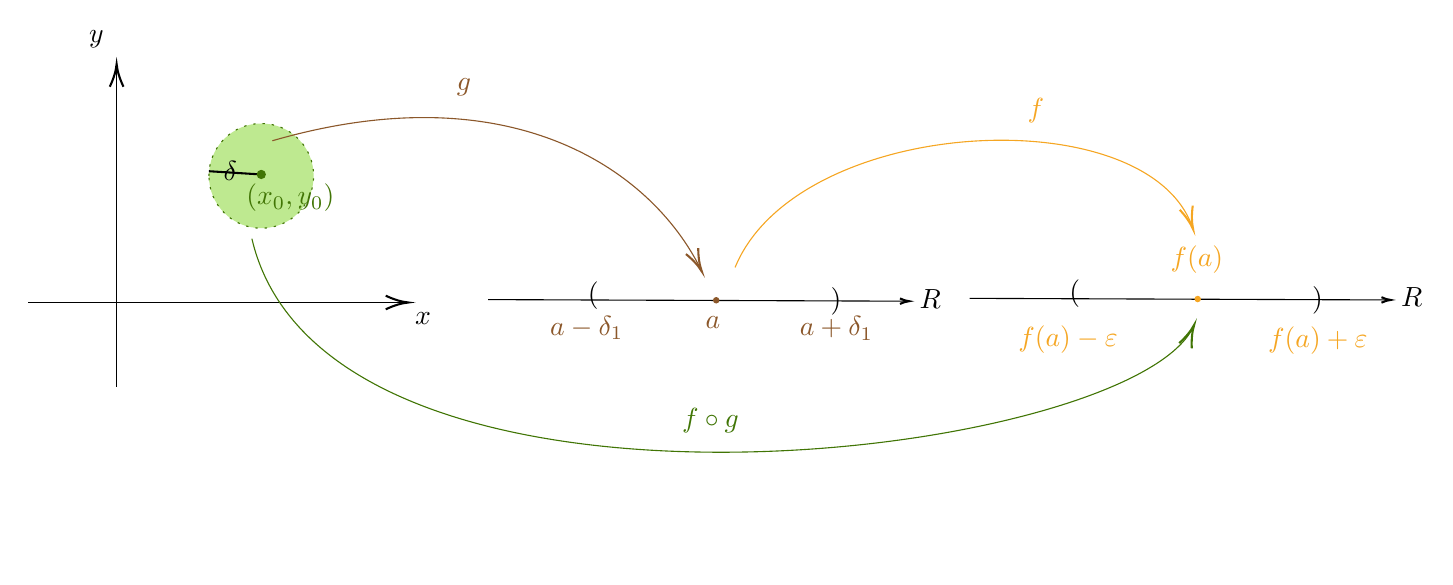
\begin{tikzpicture}[x=0.75pt,y=0.75pt,yscale=-1,xscale=1]
        % Straight Lines
        \draw (61.63,252) -- (61.63,98.5);
        \draw [shift={(61.63,96.5)}, rotate=90, color={rgb, 255:red, 0; green, 0; blue, 0}, line width=0.75] (10.93,-3.29) .. controls (6.95,-1.4) and (3.31,-0.3) .. (0,0) .. controls (3.31,0.3) and (6.95,1.4) .. (10.93,3.29);

        \draw (19.04,211.4) -- (200.2,211.4);
        \draw [shift={(202.2,211.4)}, rotate=180, color={rgb, 255:red, 0; green, 0; blue, 0}, line width=0.75] (10.93,-3.29) .. controls (6.95,-1.4) and (3.31,-0.3) .. (0,0) .. controls (3.31,0.3) and (6.95,1.4) .. (10.93,3.29);

        \draw (240.62,210) -- (441.41,210.77);
        \draw [shift={(443.41,210.78)}, rotate=180.22, color={rgb, 255:red, 0; green, 0; blue, 0}, line width=0.75] (4.37,-1.32) .. controls (2.78,-0.56) and (1.32,-0.12) .. (0,0) .. controls (1.32,0.12) and (2.78,0.56) .. (4.37,1.32);

        % Shape: Ellipse
        \draw [draw opacity=0, fill={rgb, 255:red, 139; green, 87; blue, 42}, fill opacity=1] (350.51,208.76) .. controls (351.37,208.77) and (352.06,209.47) .. (352.06,210.33) .. controls (352.06,211.19) and (351.36,211.89) .. (350.49,211.89) .. controls (349.63,211.88) and (348.94,211.18) .. (348.94,210.32) .. controls (348.94,209.46) and (349.64,208.76) .. (350.51,208.76) -- cycle;

        % Shape: Ellipse
        \draw [color={rgb, 255:red, 65; green, 117; blue, 5}, draw opacity=1, fill={rgb, 255:red, 126; green, 211; blue, 33}, fill opacity=0.5, dash pattern={on 0.84pt off 2.51pt}] (106.1,150.39) .. controls (106.1,136.46) and (117.39,125.16) .. (131.32,125.16) .. controls (145.25,125.16) and (156.55,136.46) .. (156.55,150.39) .. controls (156.55,164.32) and (145.25,175.61) .. (131.32,175.61) .. controls (117.39,175.61) and (106.1,164.32) .. (106.1,150.39) -- cycle;

        % Straight Lines
        \draw [line width=0.75] (106.1,148.15) -- (110.23,148.41) -- (131.32,149.71);

        % Shape: Circle
        \draw [draw opacity=0, fill={rgb, 255:red, 65; green, 117; blue, 5}, fill opacity=1] (129.09,149.71) .. controls (129.09,148.48) and (130.09,147.48) .. (131.32,147.48) .. controls (132.56,147.48) and (133.56,148.48) .. (133.56,149.71) .. controls (133.56,150.95) and (132.56,151.95) .. (131.32,151.95) .. controls (130.09,151.95) and (129.09,150.95) .. (129.09,149.71) -- cycle;

        % Straight Lines
        \draw (472.62,209.4) -- (673.41,210.17);
        \draw [shift={(675.41,210.18)}, rotate=180.22, color={rgb, 255:red, 0; green, 0; blue, 0}, line width=0.75] (4.37,-1.32) .. controls (2.78,-0.56) and (1.32,-0.12) .. (0,0) .. controls (1.32,0.12) and (2.78,0.56) .. (4.37,1.32);

        % Shape: Ellipse
        \draw [draw opacity=0, fill={rgb, 255:red, 245; green, 166; blue, 35}, fill opacity=1] (582.51,208.16) .. controls (583.37,208.17) and (584.06,208.87) .. (584.06,209.73) .. controls (584.06,210.59) and (583.36,211.29) .. (582.49,211.29) .. controls (581.63,211.28) and (580.94,210.58) .. (580.94,209.72) .. controls (580.94,208.86) and (581.64,208.16) .. (582.51,208.16) -- cycle;

        % Curve Lines
        \draw [color={rgb, 255:red, 139; green, 87; blue, 42}, draw opacity=1] (136.67,133.47) .. controls (252.56,99.94) and (319.58,148.18) .. (342.91,195.08);
        \draw [shift={(343.6,196.5)}, rotate=244.41, color={rgb, 255:red, 139; green, 87; blue, 42}, draw opacity=1, line width=0.75] (10.93,-3.29) .. controls (6.95,-1.4) and (3.31,-0.3) .. (0,0) .. controls (3.31,0.3) and (6.95,1.4) .. (10.93,3.29);

        % Curve Lines
        \draw [color={rgb, 255:red, 245; green, 166; blue, 35}, draw opacity=1] (359.6,194.5) .. controls (389.68,121.25) and (558.1,112.24) .. (579.98,175.2);
        \draw [shift={(580.3,176.15)}, rotate=252.24, color={rgb, 255:red, 245; green, 166; blue, 35}, draw opacity=1, line width=0.75] (10.93,-3.29) .. controls (6.95,-1.4) and (3.31,-0.3) .. (0,0) .. controls (3.31,0.3) and (6.95,1.4) .. (10.93,3.29);

        % Curve Lines
        \draw [color={rgb, 255:red, 65; green, 117; blue, 5}, draw opacity=1] (126.8,180.65) .. controls (162.62,333.88) and (549.9,287.62) .. (580.37,223.12);
        \draw [shift={(580.8,222.15)}, rotate=112.56, color={rgb, 255:red, 65; green, 117; blue, 5}, draw opacity=1, line width=0.75] (10.93,-3.29) .. controls (6.95,-1.4) and (3.31,-0.3) .. (0,0) .. controls (3.31,0.3) and (6.95,1.4) .. (10.93,3.29);

        % Text Nodes
        \draw (204.2,214.8) node [anchor=north west, inner sep=0.75pt, font=\normalsize] {$x$};
        \draw (47.17,79.26) node [anchor=north west, inner sep=0.75pt, font=\normalsize] {$y$};
        \draw (447.2,203.78) node [anchor=north west, inner sep=0.75pt, font=\normalsize] {$\mathbb{R}$};
        \draw (412.05,218.97) node [anchor=north west, inner sep=0.75pt, rotate=-180.22] {$($};
        \draw (287.45,199.91) node [anchor=north west, inner sep=0.75pt, rotate=-0.22] {$($};
        \draw (344.15,216.93) node [anchor=north west, inner sep=0.75pt, font=\normalsize, color={rgb, 255:red, 139; green, 87; blue, 42}, opacity=1] {$a$};
        \draw (122.84,153.16) node [anchor=north west, inner sep=0.75pt, font=\normalsize, color={rgb, 255:red, 65; green, 117; blue, 5}, opacity=1] {$(x_{0}, y_{0})$};
        \draw (111.94,141.93) node [anchor=north west, inner sep=0.75pt, font=\normalsize] {$\delta$};
        \draw (269.2,216.65) node [anchor=north west, inner sep=0.75pt, font=\normalsize, color={rgb, 255:red, 139; green, 87; blue, 42}, opacity=1] {$a-\delta_{1}$};
        \draw (389.54,216.98) node [anchor=north west, inner sep=0.75pt, font=\normalsize, color={rgb, 255:red, 139; green, 87; blue, 42}, opacity=1] {$a+\delta_{1}$};
        \draw (679.2,203.18) node [anchor=north west, inner sep=0.75pt, font=\normalsize] {$\mathbb{R}$};
        \draw (644.05,218.37) node [anchor=north west, inner sep=0.75pt, rotate=-180.22] {$($};
        \draw (519.45,199.31) node [anchor=north west, inner sep=0.75pt, rotate=-0.22] {$($};
        \draw (568.15,182.73) node [anchor=north west, inner sep=0.75pt, font=\normalsize, color={rgb, 255:red, 245; green, 166; blue, 35}, opacity=1] {$f(a)$};
        \draw (494.8,221.25) node [anchor=north west, inner sep=0.75pt, font=\normalsize, color={rgb, 255:red, 245; green, 166; blue, 35}, opacity=1] {$f(a)-\varepsilon$};
        \draw (615.14,221.98) node [anchor=north west, inner sep=0.75pt, font=\normalsize, color={rgb, 255:red, 245; green, 166; blue, 35}, opacity=1] {$f(a)+\varepsilon$};
        \draw (224.3,102.4) node [anchor=north west, inner sep=0.75pt] {$\textcolor[rgb]{0.55,0.34,0.16}{g}$};
        \draw (499.3,111.9) node [anchor=north west, inner sep=0.75pt] {$\textcolor[rgb]{0.96,0.65,0.14}{f}$};
        \draw (332.8,260.9) node [anchor=north west, inner sep=0.75pt] {$\textcolor[rgb]{0.25,0.46,0.02}{f\circ g}$};
    \end{tikzpicture}
    \caption{Função composta}
    \label{fig:composta}
\end{figure}

\end{proposition}

\begin{example}
    \(\displaystyle\lim_{\substack{x\to 1 \\ y\to 2}} \ln(x^2 + xy - 1) = \ln\left( \displaystyle\lim_{\substack{x\to 1 \\ y\to 2}} (x^2 + xy - 1) \right) = \ln(2). \)
\end{example}

\begin{exercise}
    Calcule os seguintes limites usando a Proposição \ref{prop.composta}
        \begin{enumerate}
            \item \(\displaystyle\lim_{\substack{x\to 0 \\ y\to \frac{\pi}{2}}} \sin(x+y) \).
            \item \(\displaystyle\lim_{\substack{x\to 0 \\ y\to 2}} \sqrt{x+y} \).
        \end{enumerate}
\end{exercise}

\section{Continuidade}

Lembre que para funções de uma variável, dizemos que \(f\) é contínua em \(x_0\in D_f\) se \[\lim_{x\to x_0} f(x) = f(x_0).\]

\begin{definition}
    Sejam \(f: D_f\subset \R^2 \to \R\) e \((x_0,y_0)\in D_f\) um ponto de acumulação de \(D_f\). Dizemos que \(f\) é contínua \index{Funções de duas variáveis a valores reais! Contínua} em \((x_0,y_0)\) se \[\displaystyle\lim_{\substack{x\to x_0 \\ y\to y_0}} f(x,y) = f(x_0,y_0). \]
\end{definition}

\begin{remark}
    Se \(f\) é contínua em todos os pontos de \(A\subset D_f\), então dizemos que \(f\) é contínua em \(A\). Em particular, se \(f\) é contínua em todos os pontos de \(D_f\), diremos simplesmente que \(f\) é contínua.
\end{remark}

\begin{exercise}
    Sejam \(f\) e \(g\) funções contínuas em \((x_0,y_0)\). Mostre que
        \begin{enumerate}
            \item \(f\pm g\) é contínua em \((x_0,y_0)\).
            \item \(f\cdot g\) é contínua em \((x_0,y_0)\).
            \item \(\frac{f}{g}\) é contínua em \((x_0,y_0)\) desde que \(g(x_0,y_0) \neq 0\).
        \end{enumerate}
\end{exercise}

\begin{example}
    \(f(x,y) = k\) é contínua em \(\R^2\). De fato, dado \((x_0,y_0)\in\R^2\), \[\displaystyle\lim_{\substack{x\to x_0 \\ y\to y_0}} f(x,y) = \displaystyle\lim_{\substack{x\to x_0 \\ y\to y_0}} k = k = f(x_0,y_0). \]
\end{example}

\begin{example}
    \(f(x,y) = x\) é contínua em \(\R^2\). De fato, dado \((x_0,y_0)\in\R^2\), temos \[\displaystyle\lim_{\substack{x\to x_0 \\ y\to y_0}} f(x,y) = \displaystyle\lim_{\substack{x\to x_0 \\ y\to y_0}} x = x_0 = f(x_0,y_0).\]
\end{example}

\begin{exercise}
    Mostre que \(f(x,y) = y\) é contínua em \(\R^2\).
\end{exercise}

\begin{example}
    \(f(x,y) = x^2\) é contínua em \(\R^2\).

    De fato, temos que \[f(x,y) = x^2 = x\cdot x,\] assim, sendo \(f\) o produto de duas funções contínuas, \(f\) é contínua.
\end{example}

\begin{exercise}
    Mostre que as seguintes funções são contínuas:
        \begin{enumerate}
            \item \(f(x,y) = x^n\), \(n\in\N\).
            \item \(f(x,y) = y^n\), \(n\in\N\).
            \item \(f(x,y) = \sum_{m+n\leq p} a_{m,n} x^my^n.\)
            \item \(f(x,y) = \frac{\sum_{m+n\leq p} a_{m,n} x^my^n}{\sum_{m+n\leq q} b_{m,n} x^my^n}\), \(a_{m,n}, b_{m,n}\in\R\).
        \end{enumerate}
\end{exercise}

\begin{example}
    Calcule \(\lim_{(x,y) \to (1,2)} (x^2y^3 - x^3y^2 + 3x + 2y)\).

    Como \(f(x,y) = x^2y^3 - x^3y^2 + 3x + 2y\) sabemos que \(\lim_{(x,y)\to(1,2)} f(x,y) = f(1,2)\), portanto \[ \lim_{(x,y) \to (1,2)} (x^2y^3 - x^3y^2 + 3x + 2y) = 1^2\cdot 2^3 - 1^3\cdot 2^2 + 3\cdot 1 + 2\cdot 2 = 11. \]
\end{example}

\begin{example}
    Estude a continuidade da função \(f(x,y) = \begin{cases}
        \frac{x^3}{x^2 + y^2},\; (x,y)\neq 0, \\
        0,\; (x,y)=(0,0).
    \end{cases}\) Sendo \(f\) o quociente de funções contínuas em \(\R^2\setminus\{(0,0)\}\), concluímos que \(f\) é contínua em \(\R^2\setminus\{(0,,0)\}\).

    Além disso, \[\displaystyle\lim_{\substack{x\to 0 \\ y\to 0}} f(x,y) = \displaystyle\lim_{\substack{x\to x_0 \\ y\to y_0}} \frac{x^3}{x^2 + y^2} = \displaystyle\lim_{\substack{x\to 0 \\ y\to 0}} x\cdot \frac{x^2}{x^2+y^2} = 0 = f(0,0). \]

    Portanto \(f\) é contínua em \(\R^2\).
\end{example}

\begin{example}
    Considere a função \[g(x,y) = \begin{cases}
        \frac{x^2 - y^2}{x^2 + y^2},\; (x,y)\neq(0,0), \\
        0,\; (x,y)=(0,0).
    \end{cases}\]

    Para \((x_0,y_0)\neq(0,0)\), \[\displaystyle\lim_{\substack{x\to x_0 \\ y\to y_0}} \frac{x^2 - y^2}{x^2 + y^2} = \frac{\displaystyle\lim_{\substack{x\to x_0 \\ y\to y_0}} (x^2 - y^2)}{\displaystyle\lim_{\substack{x\to x_0 \\ y\to y_0}} (x^2 + y^2)} = \frac{x_0^2 - y_0^2}{x_0^2 + y_0^2} = f(x_0,y_0). \] Por outro lado, já vimos que \(\displaystyle\lim_{\substack{x\to 0 \\ y\to 0}} \frac{x^2 - y^2}{x^2 + y^2} \) não existe. Portanto \(g\) é contínua em \(\R^2\setminus\{(0,0)\}\).
\end{example}

\begin{theorem}\label{thm.ContinuidadeDaComposta}
    Sejam \(g:D_g \subset \R^2 \to \R\) e \(f:D_f\subset\R^2 \to \R\) funções tais que \(\operatorname{Im}_f \subset D_g\). Se \(g\) é contínua em \((x_0,y_0)\) e \(f\) é contínua em \(g(x_0,y_0)\), então \(h(x,y) = f(g(x,y))\) é contínua em \((x_0,y_0)\).
\end{theorem}

\begin{proof}
    Dado que \(g\) é contínua em \((x_0,y_0)\), temos \[\displaystyle\lim_{\substack{x\to x_0 \\ y\to y_0}} g(x,y) = g(x_0,y_0).\] Agora, sendo \(f\) contínua em \(g(x_0,y_0)\), \[\displaystyle\lim_{\substack{x\to x_0 \\ y\to y_0}} h(x,y) = \displaystyle\lim_{\substack{x\to x_0 \\ y\to y_0}} f(g(x,y)) = f\left( \displaystyle\lim_{\substack{x\to x_0 \\ y\to y_0}} g(x,y) \right) = f(g(x_0,y_0)) = h(x_0,y_0),\] portanto \(h\) é contínua em \((x_0,y_0)\).
\end{proof}

\begin{exercise}
    Prove o Teorema \ref{thm.ContinuidadeDaComposta} utilizando as definições de limite por \(\varepsilon\) e \(\delta\).
\end{exercise}

\begin{example}
    \(h(x,y) = \sin(x^2 + 2x)\) é contínua em \(\R^2\) uma vez que \(g(x,y) = x^2 + 2x\) é contínua em \(\R^2\) e \(f(x) = \sin(x)\) é contínua em \(R\).
\end{example}

\section{Funções de 3 variáveis}

O que fizemos até agora pode ser estendido para funções de 3 (ou mais) variáveis.
\begin{enumerate}
    \item Dizemos que \(\displaystyle\lim_{\substack{x\to x_0 \\ y\to y_0 \\ z\to z_0}} f(x,y,z) = L\) se, para todo \(\varepsilon>0\), existe \(\delta>0\) tal que, para todo \((x,y,z)\in D_f\), \[0 < \|(x,y,z) - (x_0,y_0,z_0)\| \Rightarrow |f(x,y,z) - L| < \varepsilon.\]
    \item \(f:D_f\subset\R^3 \to \R\) é contínua em \((x_0,y_0,z_0)\in D_f\) se \(\displaystyle\lim_{\substack{x\to x_0 \\ y\to y_0 \\ z\to z_0}} f(x,y,z) = f(x_0,y_0,z_0)\).
\end{enumerate}